\section{Bayesian Regularized Neural Network}

Recall the regularized network weights from chapter 2. Given the posterior distribution of network weights $p(w|D,\alpha,\beta,A)$, the likelihood of new predictions $p(y^*|w,A)$, the posterior predictive distribution would be:
$$
p(y^*|x,D,\alpha,\beta,A) = \int p(y^*|w,A) p(w|D,\alpha,\beta,A) \text{ } dw
$$
which is the product the posterior distribution and the likelihood of the prediction given network weights and architecture, integrated over the weights.  This gives an output predicted distribution of $y^*$, given the same prior assumptions as went into building the model before.

This example returns to the Tohoku Earthquake problem, offering another potential solution than the MLP.  It uses the \texttt{brnn} package \cite{brnn} to fit a neural network with Bayesian regularization by means as described at the end of chapter 2 and in further detail by (Mackay, 1992).
%Data was not divided into a test set to assess predictive accuracy, although it can be in the same manner as was done earlier.  Rather than assessing predictive accuracy here, an alternate approach will be introduced.  This example serves merely as direct exposure to the regularization techniques described. The model is a two-layer Bayesian Regularized Neural Network (BRNN) to make a prediction for a magnitude 9.1 earthquake in the Tohoku area. % Its syntax is relatively simple, with many defaults that can be modified for special cases.
The models surveyed were two-layer neural networks with the same number of hidden neurons as the multi-layer perceptron.

\begin{figure}[H]
    \center
    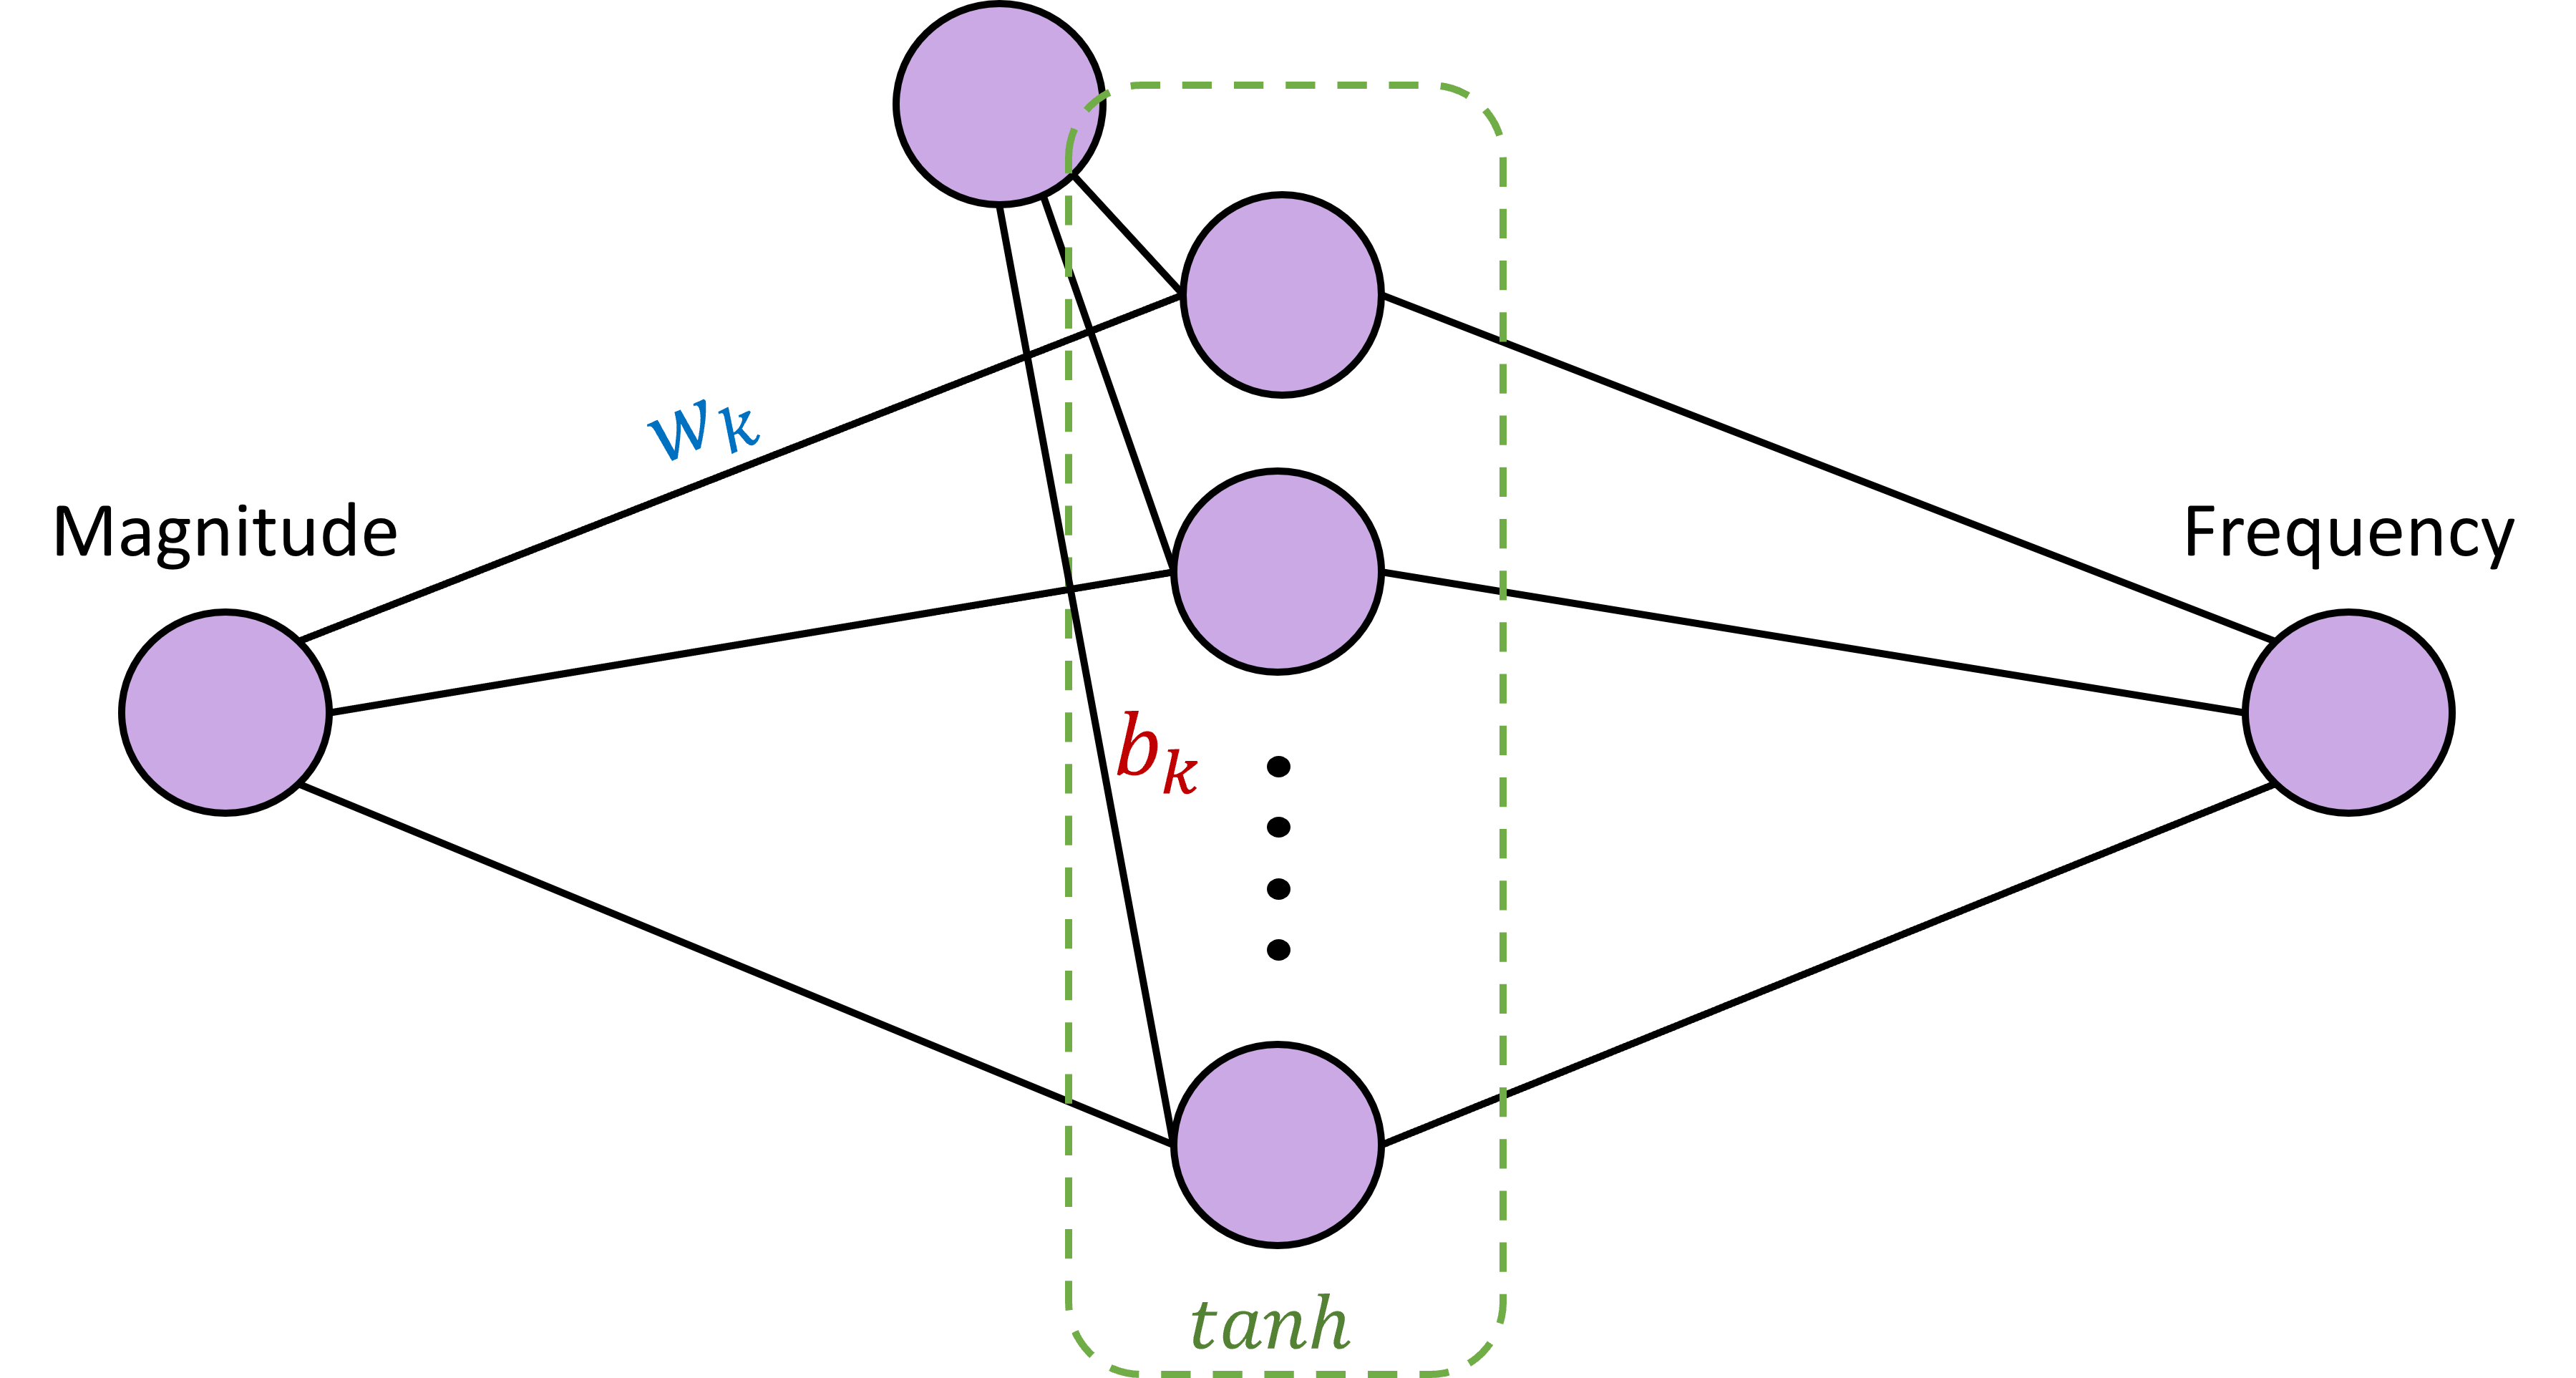
\includegraphics[width=0.55\linewidth]{Figures/BRNNdiag.png}
   % \vspace{-10pt}
    \caption{\footnotesize{Insert BRNN here}}
    \label{tohoku_unfit}
\end{figure}

By default, the \texttt{brnn} package uses hyperbolic tangent activation betwen layers and the Gauss-Newton optimization algorithm (Forsee and Hagan, 1997).  This means that is suffers the same drawbacks as the MLP model - it treats the task as a linear regression.  Only this time, it employs a regularization technique to ease the brittle nature of a high-parameter model.
Although the Gauss-Newton algorithm had little trouble converging on the standard scale, for continuity the models were built in the same manner as the multi-layer perceptron: data was transformed onto the log scale and test accuracy was measured by aggregating 50 models and determining the \textit{median} test error.

% latex table generated in R 4.2.2 by xtable 1.8-4 package
% Thu May  4 11:32:17 2023
\begin{table}[ht]
\centering
\begin{tabular}{rrr}
  \hline
\multicolumn{2}{c}{Baseline} & \multicolumn{1}{l}{Test Error} \\ 
  \hline
  \multicolumn{2}{c}{Poisson Regression Model} & \multicolumn{1}{l}{0.1862851} \\ 
  \hline
Hidden Units & Test Error (MLP) & Test Error (BRNN) \\ 
  \hline
3 & 0.2441865  & 0.1888387 \\ 
6 & 0.2818492  & 0.1949408 \\ 
9 & 0.1785652  & 0.1440102 \\ 
10 & 0.2633863  & 0.1851772 \\ 
20 & 0.1706793  & 0.1182969 \\ 
 50 & - & 0.4055160 \\ 
   \hline
\end{tabular}
   \caption{Test accuracy for all MLP and BRNN networks of different sizes compared to baseline Poisson model.}
\end{table}



Out of all network sizes tested, the best has 20 neurons in the hidden layer.  This was surprising at first, so an additional network with 50 hidden neurons was tested.  In regulating with Bayes, a complex network is shown to outperform the baseline Poisson regression model in light of few data points.  Using this neural network model, the expected frequency of any magnitude prediction has no single expected output.  Rather, because the parameters are trained using Bayes, the output estimate $\hat{y}$ comes from the posterior predictive distribution $p(y^*|x=6.1,D,\alpha,\beta,A)$.  Because this is a stochastic model, it can be generated over and over again and different predictions simulated from the same prerequisites.  Figure \ref{posteriorpredictive} shows this distribution based on 1000 network outputs 
\footnote{Note that there are \textit{only} 1000 predictions, so the distribution is a rough approximations.  With more attempts, or by means of other approximation techniques like those described earlier, a more accurate distributional estimate could be attained.}
 from the two-layer BRNN with 20 hidden neurons.

\begin{figure}[H]
    \center
    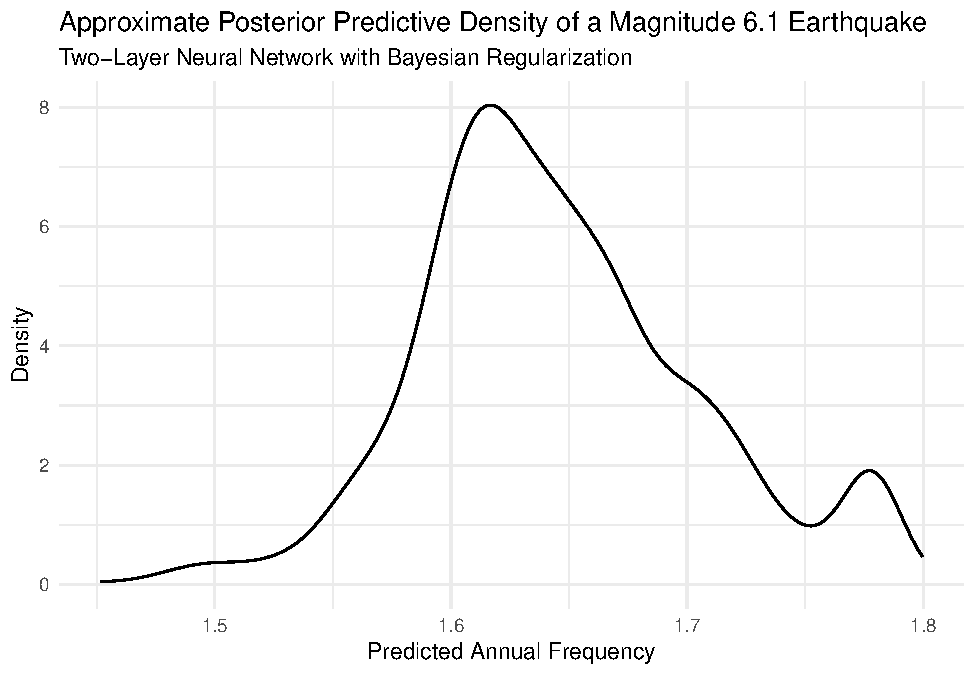
\includegraphics[width=0.75\linewidth]{Appendix_eq_files/figure-latex/unnamed-chunk-17-1.pdf}
   % \vspace{-10pt}
    \caption{\footnotesize{Simulated predictive outputs for a magnitude 6.1 earthquake from the BRNN model}}
    \label{posteriorpredictive}
\end{figure}

The model describes the expected annual frequency of a magnitude 6.1 earthquake in the Tohoku region to be somewhere between 1.4 and 1.8 per year.  Most of the density is around 1.6-1.7 per year.  By use of Bayes, the entire distribution is used to tell the story.